% https://texample.net/tikz/examples/yin-and-yang/
% Preamble
\documentclass[11pt]{article}

% Packages
\usepackage{amsmath}
\usepackage{tikz}
\usepackage{xcolor}

% Document
\begin{document}
    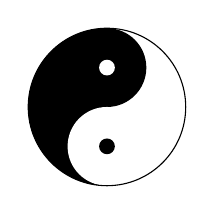
\begin{tikzpicture}
        %color one half of a unit circle
        \begin{scope}
          \clip (0,0) circle (1cm);
          \fill[black] (0cm,1cm) rectangle (-1cm, -1cm);
        \end{scope}

        %fill heads
        \fill[black] (0,0.5) circle (0.5cm);
        \fill[white] (0,-0.5) circle (0.5cm);

        %fill eyes
        \fill[white] (0,0.5) circle (0.1cm);
        \fill[black] (0,-0.5) circle (0.1cm);

        %outer line
        \draw (0,0) circle (1cm);
    \end{tikzpicture}

    \definecolor{lightOrange}{HTML}{E67E29}
    \definecolor{darkBlue}{HTML}{20154F}
    \begin{tikzpicture}
        %color one half of a unit circle
        \begin{scope}
          \clip (0,0) circle (1cm);
          \fill[lightOrange] (0cm,1cm) rectangle (-1cm, -1cm);
        \end{scope}
        \begin{scope}
          \clip (0,0) circle (1cm);
          \fill[darkBlue] (0cm,-1cm) rectangle (1cm, 1cm);
        \end{scope}

        %fill heads
        \fill[lightOrange] (0,0.5) circle (0.5cm);
        \fill[darkBlue] (0,-0.5) circle (0.5cm);

        %fill eyes
        \fill[darkBlue] (0,0.5) circle (0.1cm);
        \fill[lightOrange] (0,-0.5) circle (0.1cm);
    \end{tikzpicture}
\end{document}
